\documentclass{article}

%%  Packages
\usepackage{fullpage}
\usepackage[top=2cm, bottom=3cm, left=2.5cm, right=2.5cm]{geometry}
\usepackage{amsmath,amsthm,amsfonts,amssymb,amscd}
\usepackage{lastpage}
\usepackage{enumerate}
\usepackage{fancyhdr}
\usepackage{mathrsfs}
\usepackage{xcolor}
\usepackage{graphicx}
\graphicspath{ {images/} }
\usepackage{listings}
\usepackage{hyperref}
\usepackage{tikz}
\usetikzlibrary{decorations.markings,
		automata,
                positioning,
                quotes}
\usepackage{mathtools}
\usepackage{breqn}
\usepackage{tensor}
\usepackage{pgfplots}
\usepackage{changepage}
\usepackage[]{mdframed}
\usepackage[shortlabels]{enumitem}
\usepackage{dsfont}
\usepackage{blkarray}
\usepackage{titlesec}

\pgfplotsset{compat=1.18, width=10cm}

%%  Commands
\newcommand{\R}{\mathbb{R}}
\renewcommand{\P}{\mathbb{P}}
\newcommand{\E}{\mathbb{E}}
\newcommand{\Rar}{\Rightarrow}
\newcommand{\Var}{\text{Var}}
\newcommand{\Cov}{\text{Cov}}
\renewcommand{\vec}[1]{\underline{#1}}
\newcommand{\mat}[1]{\underline{\underline{#1}}}

%Various possibilities for "types" of question
\theoremstyle{definition}
\newtheorem*{prob}{Problem}
\newenvironment{sol}{\noindent \underline{Solution}:}
%{\qed}

%%  Page Setup
\pagestyle{plain}

\linespread{1.5}

\titlespacing*{\section}{0pt}{0pt}{0pt}

\begin{document}

\setlength{\parindent}{0pt}
\setlength{\parskip}{8pt}
\renewcommand\qedsymbol{$\blacksquare$}

\makeatletter
\renewcommand*\env@matrix[1][\arraystretch]{%
  \edef\arraystretch{#1}%
  \hskip -\arraycolsep
  \let\@ifnextchar\new@ifnextchar
  \array{*\c@MaxMatrixCols c}}
\makeatother

\title{Portfolio Optimization via Markowitz Model Extensions}
\author{Jake Merry}
\maketitle

% ---------------- %
%   Introduction   %
% ---------------- %
\section{Introduction}

In 1952, Harry Markowitz published a paper in the \emph{Journal of Financial} under the title ``Portfolio Selection''. In this paper, Markowitz first presented his optimization model that would define what is known as modern portfolio theory, and for which he would later win the Nobel Memorial Prize in Economic Sciences. We will build off Markowitz's ideas to optimize a simple stock portfolio, comparing different extensions as we go to ensure that we choose a good model for our data. 

To achieve the Markowitz model, we start with an index set $\Omega = \{ 1, 2, \dots, n \}$ of financial assets which we call our universe. We associate with our universe a probability vector $\vec\omega$ such that for all $i \in \Omega$, $\omega_i$ is the proportion of our total wealth that we invest in asset $i$. 

With respect to any universe, there exists a random vector $(R^{(1)}, R^{(2)}, \dots, R^{(n)})$ where each $R^{(i)}$ represents the return of an asset $i \in \Omega$. Then, for each $i \in \Omega$, we can define $\mu_i = \E(R^{(i)})$, the expected value of the return price of asset $i$. However, we are more interested in the total return of our entire portfolio, given by
$$R = \sum_{i \in \Omega} \omega_i R^{(i)}.$$
We can then find the total expected return of our portfolio as follows:
$$\E(R) = \E\left( \sum_{i \in \Omega} \omega_i R^{(i)} \right) = \sum_{i \in \Omega} \omega_i \E(R^{(i)}) = \sum_{i \in \Omega} \omega_i \mu_i = \vec\mu^T\omega.$$
Similarly, we can solve for the total variance of the returns:
$$\Var(R) = \Var\left( \sum_{i \in \Omega} \omega_i R^{(i)} \right) = \sum_{i, j \in \Omega} \Cov(\omega_i R^{(i)}, \omega_j R^{(j)}) = \sum_{i, j \in \Omega} \omega_i \omega_j \Cov(R^{(i)}, R^{(j)}) = \vec\omega^T \mat\Sigma \, \vec\omega, $$
where $\mat\Sigma$ is the covariance matrix of the returns vector. 

One common form of the Markowitz model is the constant expected returns (CER) model. To derive this model, we start by chosing a return rate $R$ which we will hold constant while we minimize the risk to our investment. In other words, our goal is to find the weights $\vec\omega^*$ which minimizes the variance of the returns of our portfolio, while having a constant return rate of $R$. 

The CER model is, hence, defined as follows:
\begin{align*}
	\text{minimize} \quad & \vec\omega^T \mat\Sigma \, \vec\omega \\	
	\text{subject to} \quad & \vec\mu^T \vec\omega = R \\
				& \vec 1^T \vec\omega = 1.
\end{align*}
This is the model that we will work with in this report. 


% ------------ %
%   Analysis   %
% ------------ %

\section{Analysis}

We begin by collecting stock data for the top 20 companies on the S\&P 500 by weight. Data was collected monthly from nasdaq.com starting from May 1999. Then, for each asset in our portfolio, we have a collection of numbers $\{ P_t^{(i)} \}$, representing the price of asset $i \in \Omega$ at a time $t$. We convert the prices to returns via the following formula:
$$R_t^{(i)} = \frac{P_t^{(i)} - P_{t-1}^{(i)}}{P_{t-1}^{(i)}}.$$
Taking the sample mean and covariances of each collection, we define 
$$\hat\mu_i = \frac{1}{m} \sum_{t=1}^m R_t^{(i)} \quad \text{and} \quad \hat\Sigma_{ij} = \frac{1}{m-1} \sum_{t=1}^m (R_t^{(i)} - \hat\mu_j)(R_t^{(j)} - \hat\mu_k).$$
Hence, we have the sample mean vector $\hat\mu = (\hat\mu_1, \dots, \hat\mu_n)$ and sample covariance matrix 
$$\hat\Sigma = \begin{bmatrix}[0.7]
	\hat\Sigma_{11} & \dots & \hat\Sigma_{1n} \\
	\vdots & \ddots & \vdots \\
	\hat\Sigma_{m1} & \dots & \hat\Sigma_{mn}
\end{bmatrix},$$
which we will use in place of $\mu$ and $\Sigma$ in our analysis. 

\subsection{Vanilla Model}

The first thing we notice about our derived model is that it does not include a nonnegativity constraint. Although this means that our optimal weight vector $\vec\omega^*$ may have negative components, this is not an accident. It may seem that, if this were to happen, that our model is telling us to take money from these assets and invest that money in other assets. But how is this possible? What a negative optimal weight really refers to is that this model allows for a technique called shorting. Shorting an asset is when an investor buys shares of that asset from a broker and sells them in an open market with the hope of later buying them back at a lower price and collecting on the difference. 

Assuming that we continue with this model, computation is very simple. We define the Lagrangian of this problem as 
$$\ell(\omega, \lambda) = \vec\omega^T \mat\Sigma \, \vec\omega + \lambda_1 (\vec\mu^T \vec\omega - R) + \lambda_2 (\vec 1^T \vec\omega - 1).$$
Then, we can define the second-order sufficient conditions for our model as below.

Suppose there exists some pair $(\vec\omega^*, \vec\lambda^*)$ such that the following conditions hold: 
\begin{enumerate}
	\item $\nabla_{\omega} \ell(\vec\omega^*, \vec\lambda^*) = 2\mat\Sigma\,\vec\omega^* + \lambda_1^* \vec\mu + \lambda_2^* \vec{1} = 0$,
	\item $\vec{y}^T\nabla_{\omega\omega}^2\ell(\vec\omega^*, \vec\lambda^*)\vec{y} = 2\vec{y}^T \mat\Sigma \, \vec{y} > 0$ for all $\vec{y} \in T(\vec\omega^*)$,
	\item $\vec\mu^T \vec\omega^* = R$,
	\item $\vec 1^T \vec\omega^* = 1$.
\end{enumerate}
Then $\omega^*$ is a strict local minimizer. Hence, we look for a vector $(\vec\omega, \lambda_1, \lambda_2)$ such that 
$$\begin{bmatrix}[0.7]
	2\mat\Sigma & \vec\mu & \vec{1} \\
	\vec\mu^T & 0 & 0 \\
	\vec{1}^T & 0 & 0 \\
\end{bmatrix} \begin{bmatrix}[0.7] \vec\omega \\ \lambda_1 \\ \lambda_2 \end{bmatrix} = 
\begin{bmatrix}[0.7]
	0 \\ R \\ 1
\end{bmatrix}.$$
\begin{minipage}{0.5\textwidth}
We see that this problem can be solved using linear algebra alone, and although solving would involve the computation of a potentially large matrix inverse, this problem is very nice. Solving for all $R \in [0, 0.10]$, we plot the minimized risk against the return rate to find what is called the efficient frontier of our portfolio. 
\end{minipage}
\begin{minipage}{0.49\textwidth}
	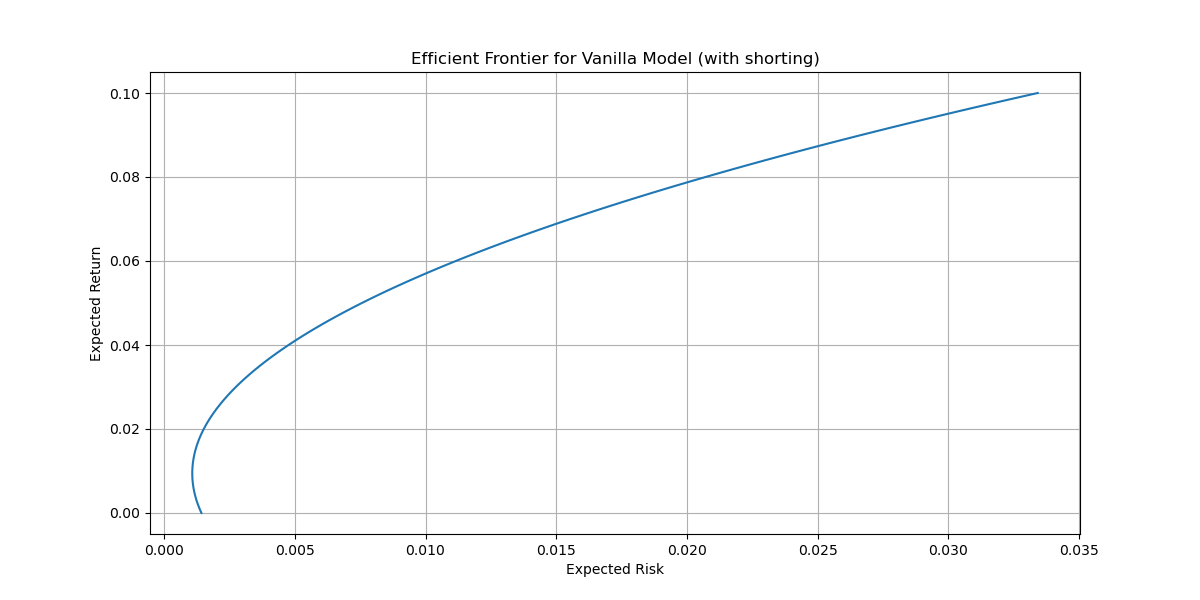
\includegraphics[width=\textwidth]{shortModel.png}
\end{minipage}

However, allowing shorting in our model can introduce more risk than the objective function accounts for. Therefore, it would be beneficial under our circumstances to require nonnegativity, i.e. add the constraint $\vec\omega \geq 0$ to our model. Although this problem can no longer be solved by linear algebra alone, we now obtain a quadratic program whose second-order sufficient conditions are the same the previous problem with the addition of the nonnegativity constraint. 

In terms of feasibility, the original problem had optimal solutions for all $R$ since the problem could be solved using a matrix computation. However, with the nonnegativity constraint, we find that it is impossible to achieve a feasible solution for any $R > \max_i\{\mu_i\}$ since we would require $\vec\mu^T\vec\omega > \max_i\{\mu_i\}$ with $\vec 1^T \vec\omega = 1$ and $\vec\omega \geq 0$. Similarly, there is no feasible solution for $R < \min_i\{\mu_i\}$. Hence, we restrict our problem to $R \in [\min_i\{ \mu_i \}, \max_i\{ \mu_i \}]$. With this in mind, we plot the efficient frontier for the new, no shorting model and compare it with the original model. 

\begin{minipage}{0.49\textwidth}
\begin{center}
	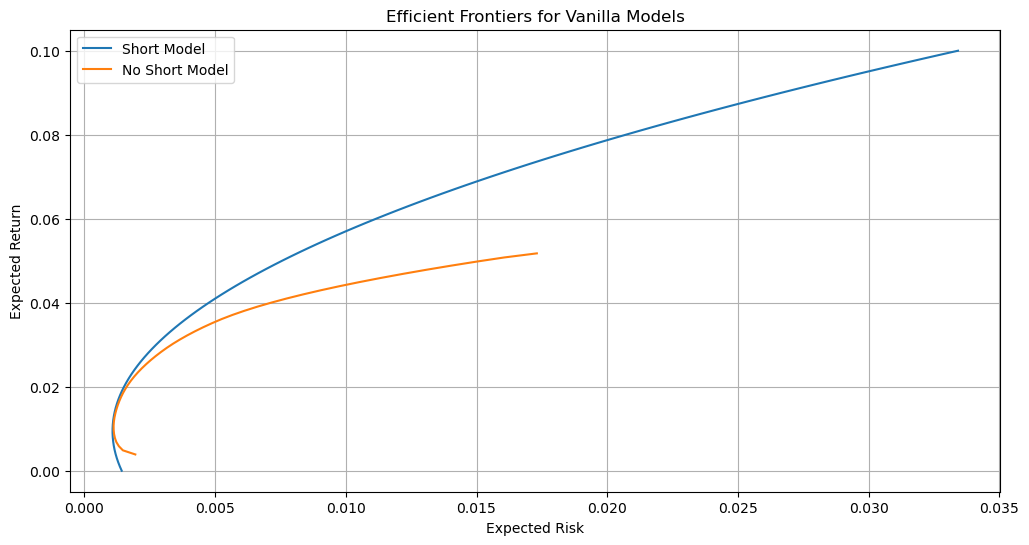
\includegraphics[width=0.9\textwidth]{shortVsNoShort.png}
\end{center}
\end{minipage}
\begin{minipage}{0.5\textwidth}
Although the efficient frontier for the model without shorting falls entirely beneath that of the model which allows shorting, we will continue our analysis with the nonnegativity constraint due to the complicated nature of shorting. 
\end{minipage}


\subsection{Risk-Free Asset Model}

We now introduce our first extension of the Markowitz model. We construct a risk-free asset model by adding to our previous model an extra asset whose return variance is (close to) zero. This asset typically represents cash, so we will denote it as $\omega_{cash}$. We update the constraints of our model to 
$$\vec\mu^T \vec\omega + r_f \omega_{cash} = R, \quad \vec 1^T \vec\omega + \omega_{cash} = 1, \quad \vec\omega, \omega_{cash} \geq 0 \qquad (r_f \text{ small})$$
and solve for the efficient frontier.

\begin{minipage}{0.5\textwidth}
Since the form of the problem has not changed by adding the extra asset, we solve the program in the same way as before. Then, we can plot the efficient frontier for the risk-free asset model and compare it to the no shorting model from before. 
\end{minipage}
\begin{minipage}{0.49\textwidth}
\begin{center}
	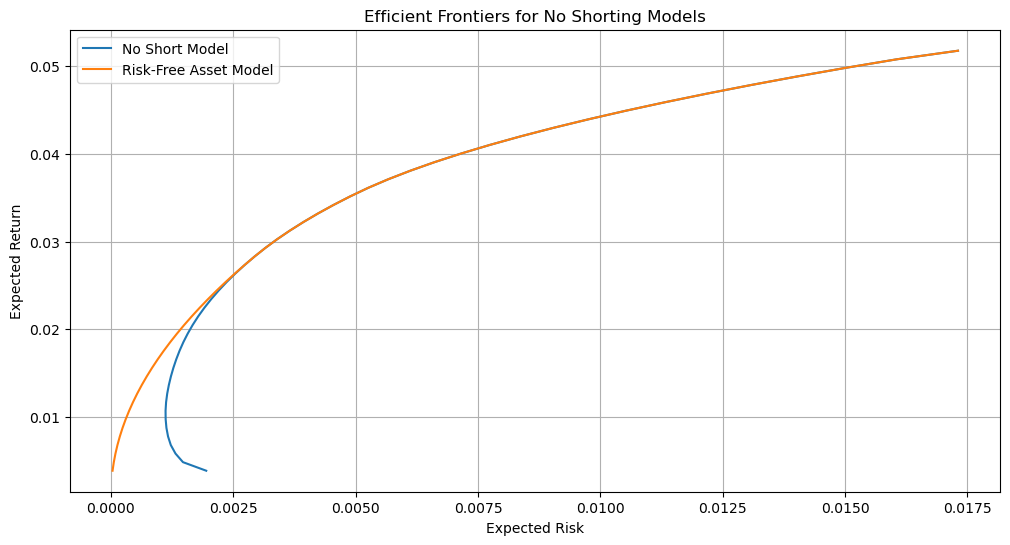
\includegraphics[width=0.8\textwidth]{noShortVsRiskFreeAsset.png}
\end{center}
\end{minipage}

Our model has the expected result of extending the previous efficient frontier to one in which a portfolio exists such that the return and variance of the investment are both (close to) zero. 

\subsection{Comparison of Penalties}

For the final part of our project, we will compare the constructed model to those with different added penalty terms to see if any of them benefit our model. Specifically, we will compare the $\ell_1$ norm for sparsity and the square of the $\ell_2$ norm for data sensitivity. The models, respectively, have objective functions 
$$\vec\omega^T \mat\Sigma \, \vec\omega + \gamma||\vec\omega||_1 \quad \text{and} \quad \vec\omega^T \mat\Sigma \, \vec\omega + \gamma||\vec\omega||_2^2,$$
where $\gamma \geq 0$. For our analysis, we choose a small set of potential $\gamma$ values and plot all efficient frontiers against that of the standard risk-free asset model. Here are the results:
\begin{center}
	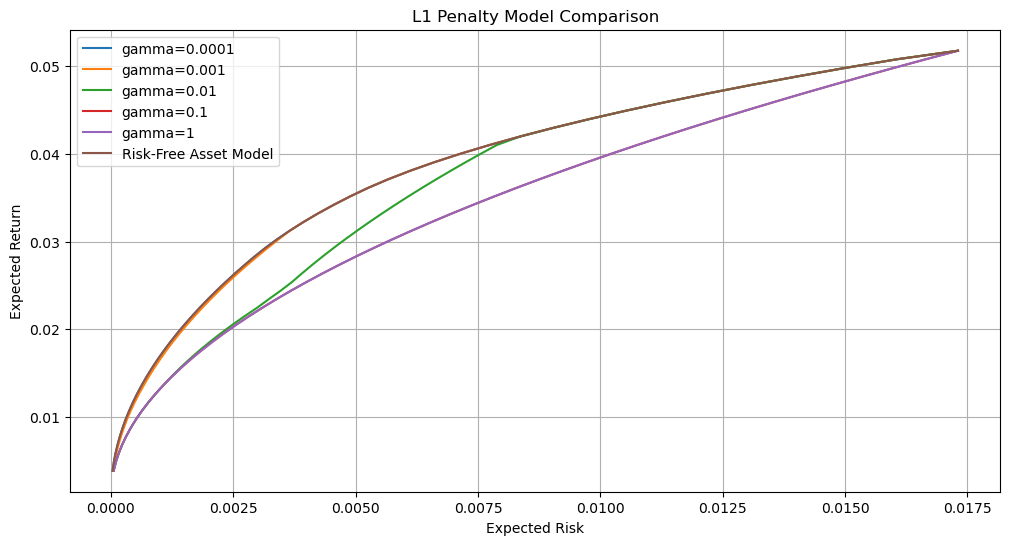
\includegraphics[width=0.48\textwidth]{L1.png}
	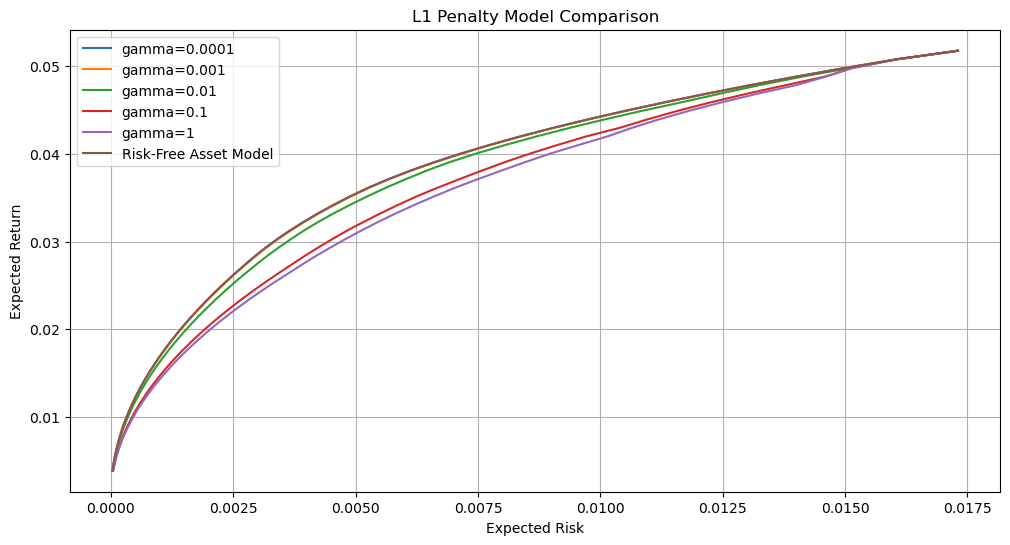
\includegraphics[width=0.48\textwidth]{L2.png}
\end{center}
We see that neither penalty decreases the variance of a portfolio at a fixed return rate, but this does not mean that these models are entirely invalid. Both penalties have models that, at very low values of $\gamma$ are nearly identical to the original model, but would add other, potentially beneficial characteristics to our model. 


\section{Conclusion}

After testing multiple different extensions, we found the best model for our data to be that of the risk-free asset model with no added penalty terms. This model behaved as expected, extending the efficient frontier of the no shorting model to the origin, but when we attempt to add an $\ell_1$ or $\ell_2$ norm penalty term to the model, the efficient frontier moved in a negative direction. This would return portfolios with the same expected return rate at a higher variance level. 

\begin{thebibliography}{}

\bibitem{wyss}
Portfolio Optimization: Notes by Justin Wyss-Gallifent

\bibitem{chong}
Chong, E. K.P., Lu, W., \& Zak, S. H. (2024). \emph{An Introduction to Optimization with Applications to Machine Learning}. John Wiley \& Sons, Inc. 

\bibitem{recht}
Wright, S. J., \& Recht, B. (2022). \emph{Optimization for Data Analysis}. Cambridge University Press. 

\bibitem{atz}
An Introduction to Portfolio Theory: Notes by Paul Atzberger

\bibitem{data}
Nasdaq, \href{www.nasdaq.com/}{www.nasdaq.com/}. Accessed 28 May 2025. 

\end{thebibliography}


\end{document}
